%\section{Appendix}


\chapter{Appendix} \label{anhang_1}


\begin{algorithm}
\caption{3D Post-processing and Mask Reconstruction}
\label{algo:maskrecon}
\begin{algorithmic}[1]
\STATE \textbf{Input:} Flow field $\mathbf{dP} \in \mathbb{R}^{3 \times L_z \times L_y \times L_x}$, probability map $\mathbf{P} \in [0,1]^{L_z \times L_y \times L_x}$, thresholds $\tau_p, \tau_s$, iterations $T$
\STATE \textbf{Output:} Segmentation volume $M$
\STATE Identify foreground voxels: $\Omega = \{ (z,y,x) \mid \mathbf{P}(z,y,x) > \tau_p \}$
\FOR{each voxel $(z,y,x) \in \Omega$}
    \STATE Initialize $\mathbf{p}_0 \gets$ normalized position of $(z,y,x)$
    \FOR{$t = 0$ to $T-1$}
        \STATE Update position: $\mathbf{p}_{t+1} \gets \mathrm{clip}(\mathbf{p}_t + \mathbf{dP}(\mathbf{p}_t), -1, 1)$
    \ENDFOR
    \STATE Store final position $\mathbf{p}_T$
\ENDFOR
\STATE Initialize histogram $H(\mathbf{u}) = 0$
\FOR{each voxel $i$ with final position $\mathbf{p}_T^{(i)}$}
    \STATE Increment histogram: $H(\mathbf{p}_T^{(i)}) \gets H(\mathbf{p}_T^{(i)}) + 1$
\ENDFOR
\STATE Detect local maxima in $H$ using $n$D max pooling (kernel size = 5)
\STATE Retain peaks with counts above threshold as seeds
\FOR{each seed $s$}
    \STATE Initialize seed mask in $11 \times 11 \times 11$ neighborhood
    \STATE Expand by morphological max pooling under constraint $H(\mathbf{u}) > 2$
\ENDFOR
\FOR{each voxel $i \in \Omega$}
    \STATE Assign voxel to label $m$ of corresponding seed region
\ENDFOR
\FOR{each mask}
    \IF{mask size $> \tau_s \cdot$ image volume} 
        \STATE Discard mask
    \ELSIF{mask size $<$ min\_size}
        \STATE Remove and fill mask
    \ELSIF{flow-consistency is low}
        \STATE Prune mask
    \ENDIF
\ENDFOR
\STATE Renumber masks to enforce consecutive labels $\{1,\dots,N\}$
\RETURN $M$
\end{algorithmic}
\end{algorithm}


\begin{figure}[!ht]
    \centering
    \makebox[\textwidth]{%
    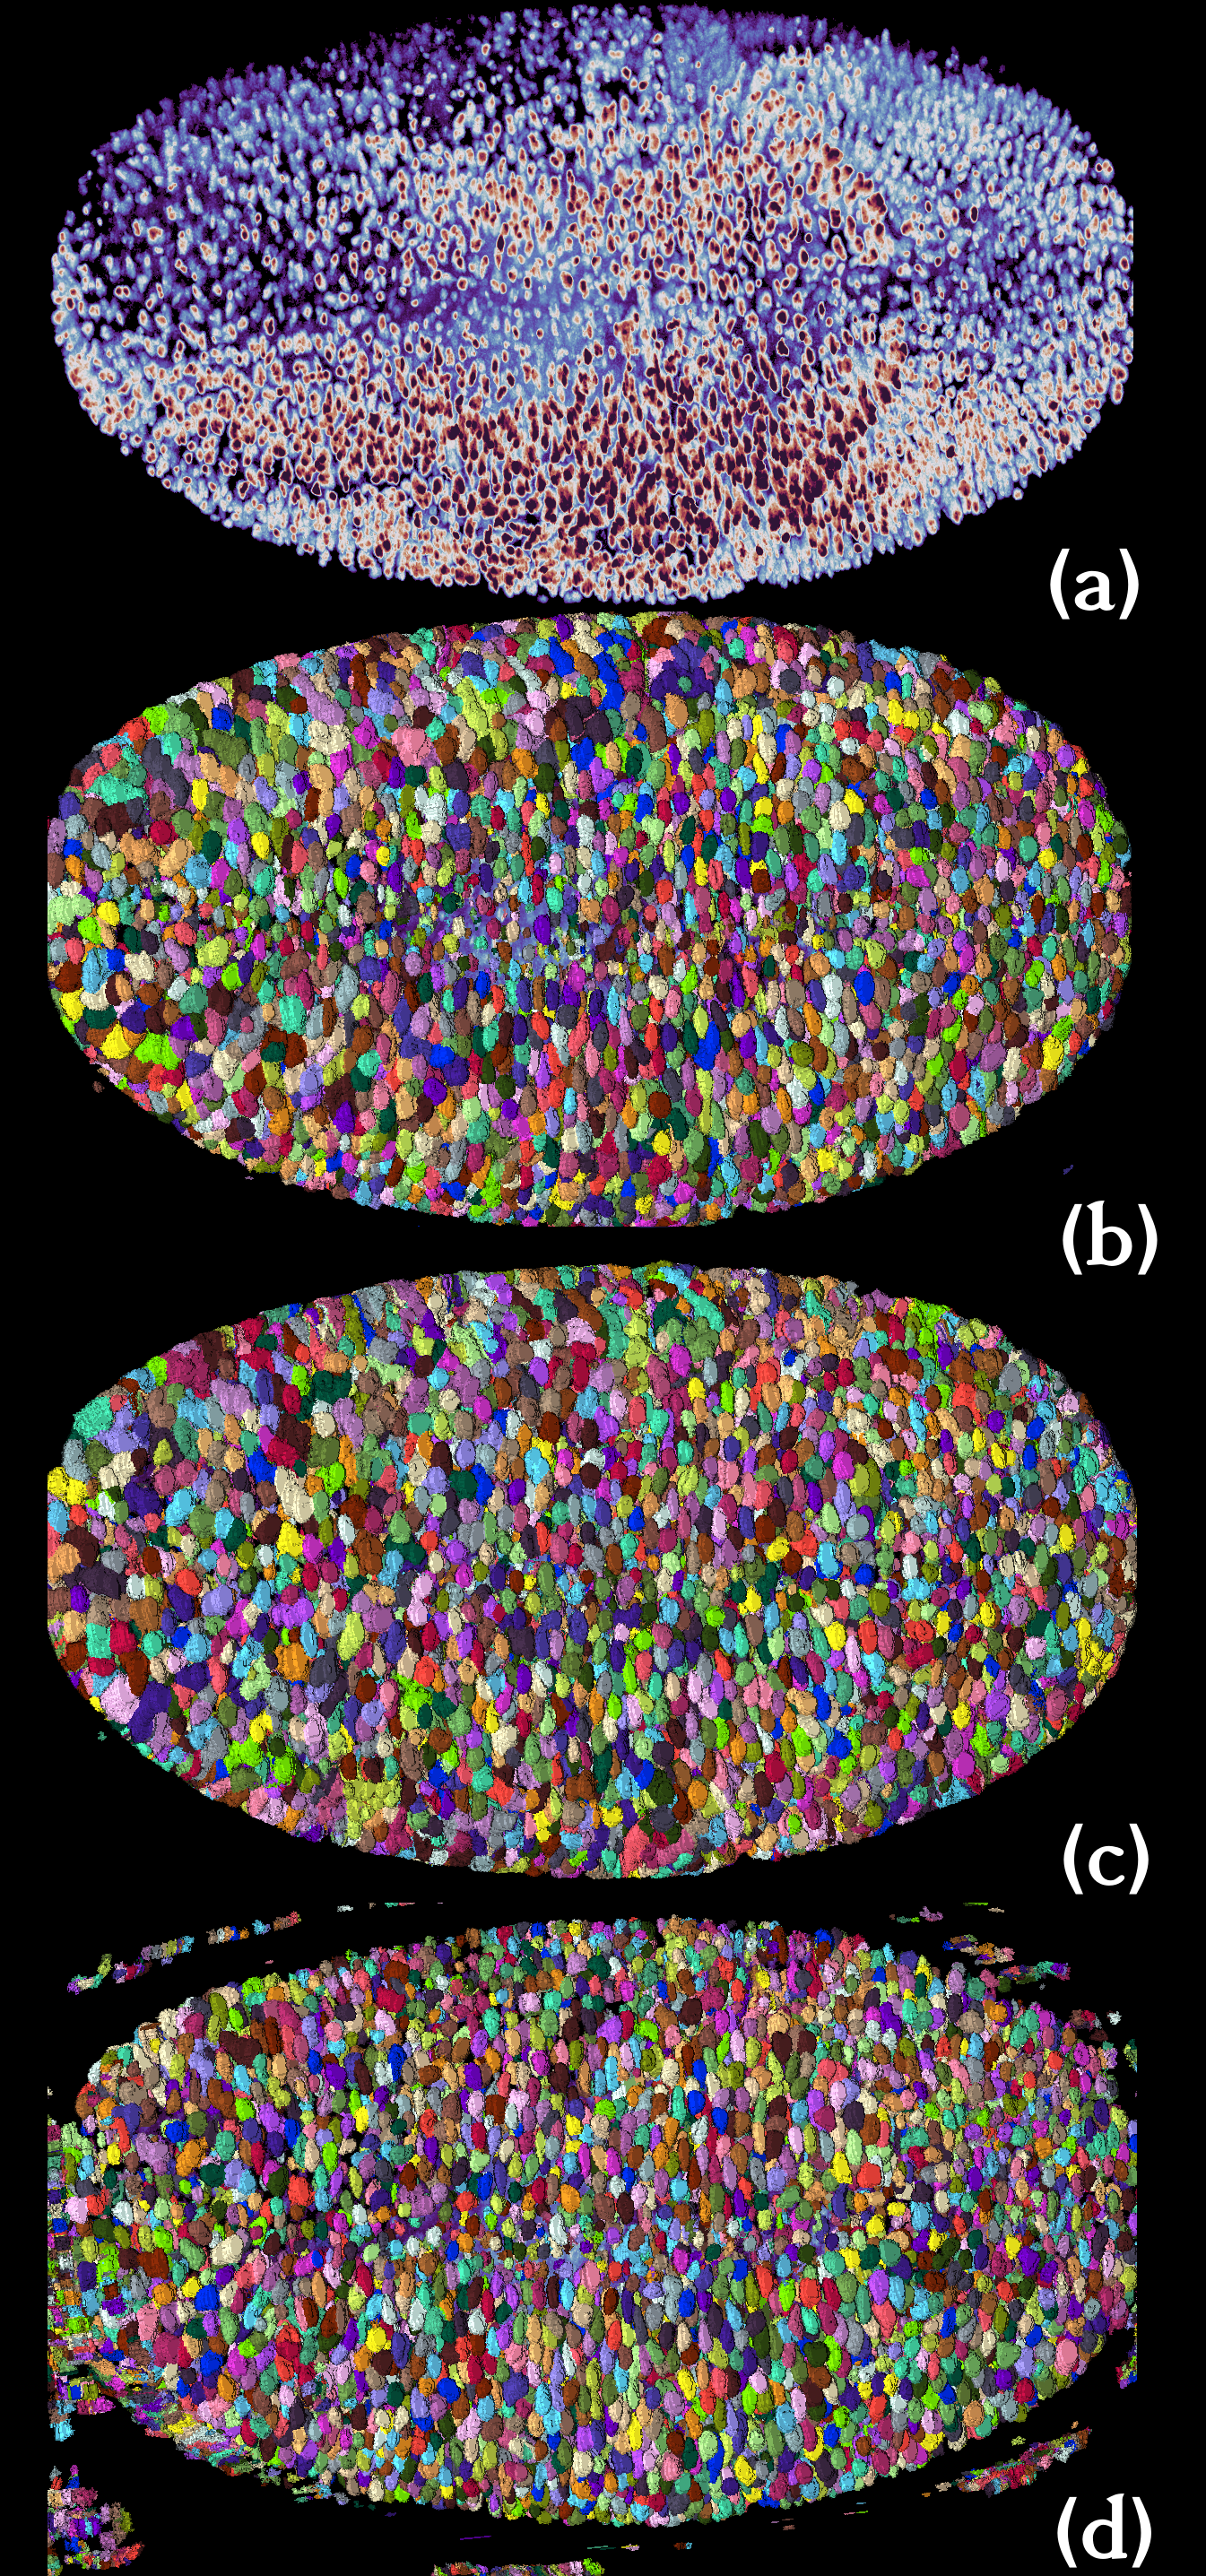
\includegraphics[width=0.6\textwidth]{Images/Appendix/DRO_3D_VIS.png}%
    }
    \caption{3D Renderings of DRO 02 sequence, timestamp 000. All models have been trained on 1000 ROIs with masked loss. a: original image, b: Mediar3D + ext. pretraining (0.72 SEG), c: Mediar3D + SAM2 Encoder (0.72 SEG), d: Mediar3D + paper weights (0.78 SEG). Artifacts in this prediction are probably due to clipping edges from manual image cropping around the primordium, done by the challenge authors for smaller file sizes.}
    \label{fig:DRO_3D_VIS}
\end{figure}


\begin{figure}[!ht]
    \centering
    \makebox[\textwidth]{%
    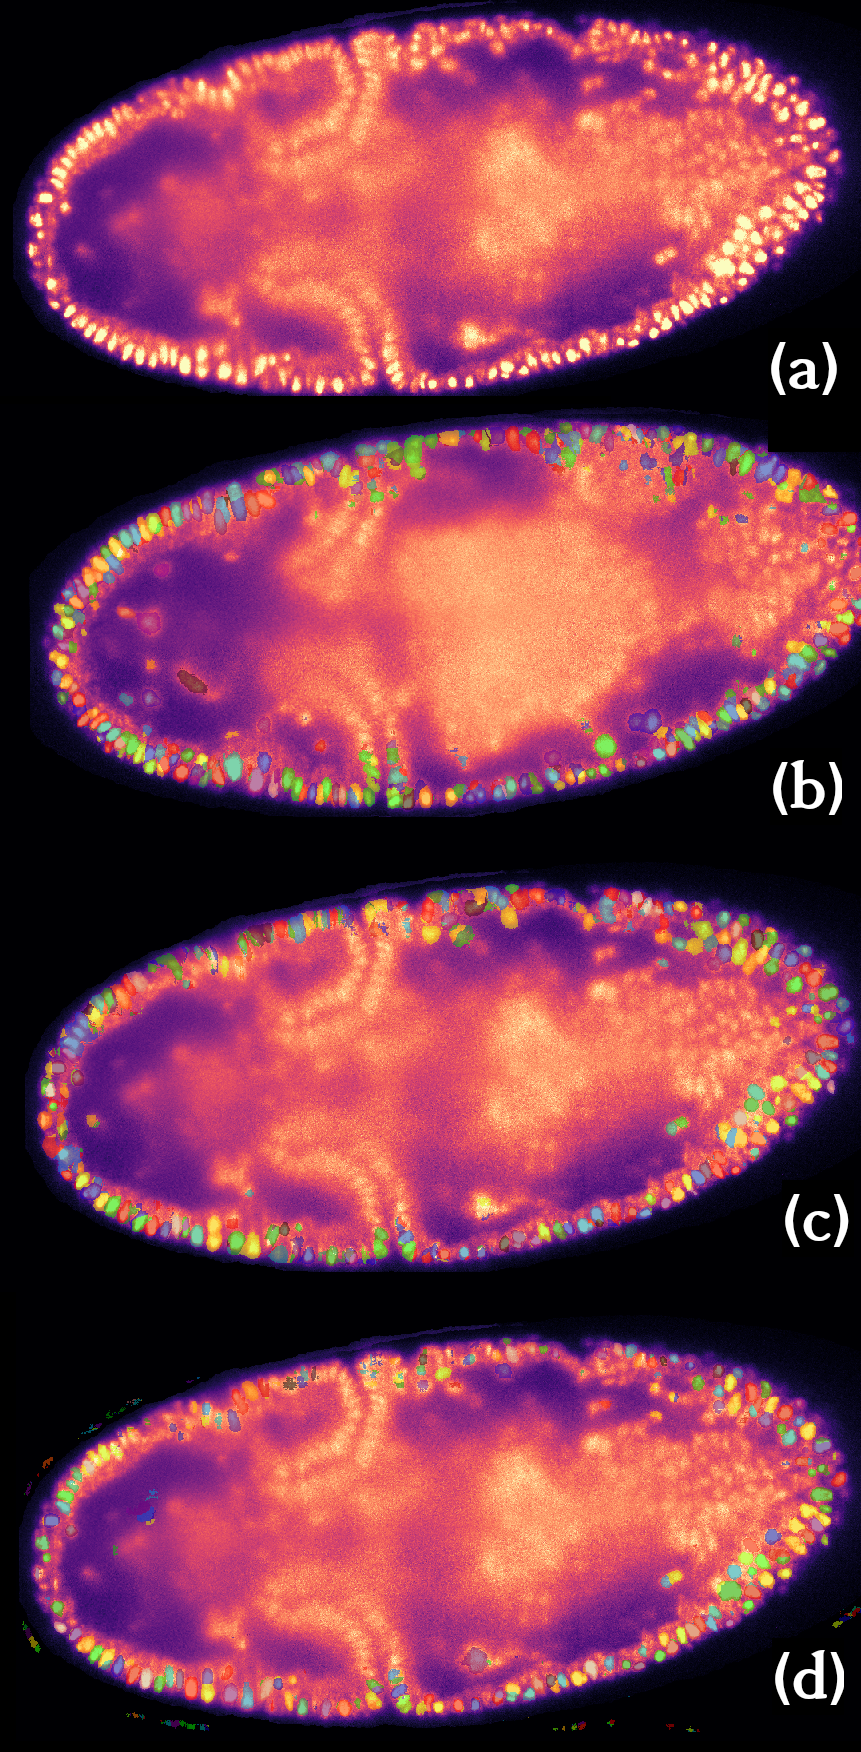
\includegraphics[width=0.63\textwidth]{Images/Appendix/DRO_2D_VIS.png}%
    }
    \caption{Z-slice 52 prediction overlays of DRO 02 sequence, timestamp 000. All models have been trained on 1000 ROIs with masked loss. a: original image, b: Mediar3D + ext. pretraining (0.72 SEG), c: Mediar3D + SAM2 Encoder (0.72 SEG), d: Mediar3D + paper weights (0.78 SEG). Artifacts in this prediction are probably due to clipping edges from manual image cropping around the primordium, done by the challenge authors for smaller file sizes.}
    \label{fig:DRO_2D_Vis}
\end{figure}

\begin{figure}[!ht]
    \centering
    \makebox[\textwidth]{%
    \includegraphics[width=1.0\textwidth]{Images/Appendix/DRO_2D_zeroshot_Vis.png}%
    }
    \caption{Zeroshot predictions on z-slice 52 of DRO 02 sequence, timestamp 000. a: Original Image, b: Mediar3D + ext. pretraining (0.74 SEG), c: Mediar3D + SAM2 Encoder (0.66 SEG), d: Mediar3D + paper weights (0.78 SEG), e: CellposeSAM (No SEG, as SEG is calculated as average from all labeled instances across all timestamps in the 02 sequence. Predicting all timestamps in the 02 sequence would be too expensive due to high inference time for CellposeSAM).}
    \label{fig:DRO_2D_zeroshot_Vis}
\end{figure}


\begin{figure}[!ht]
    \centering
    \makebox[\textwidth]{%
    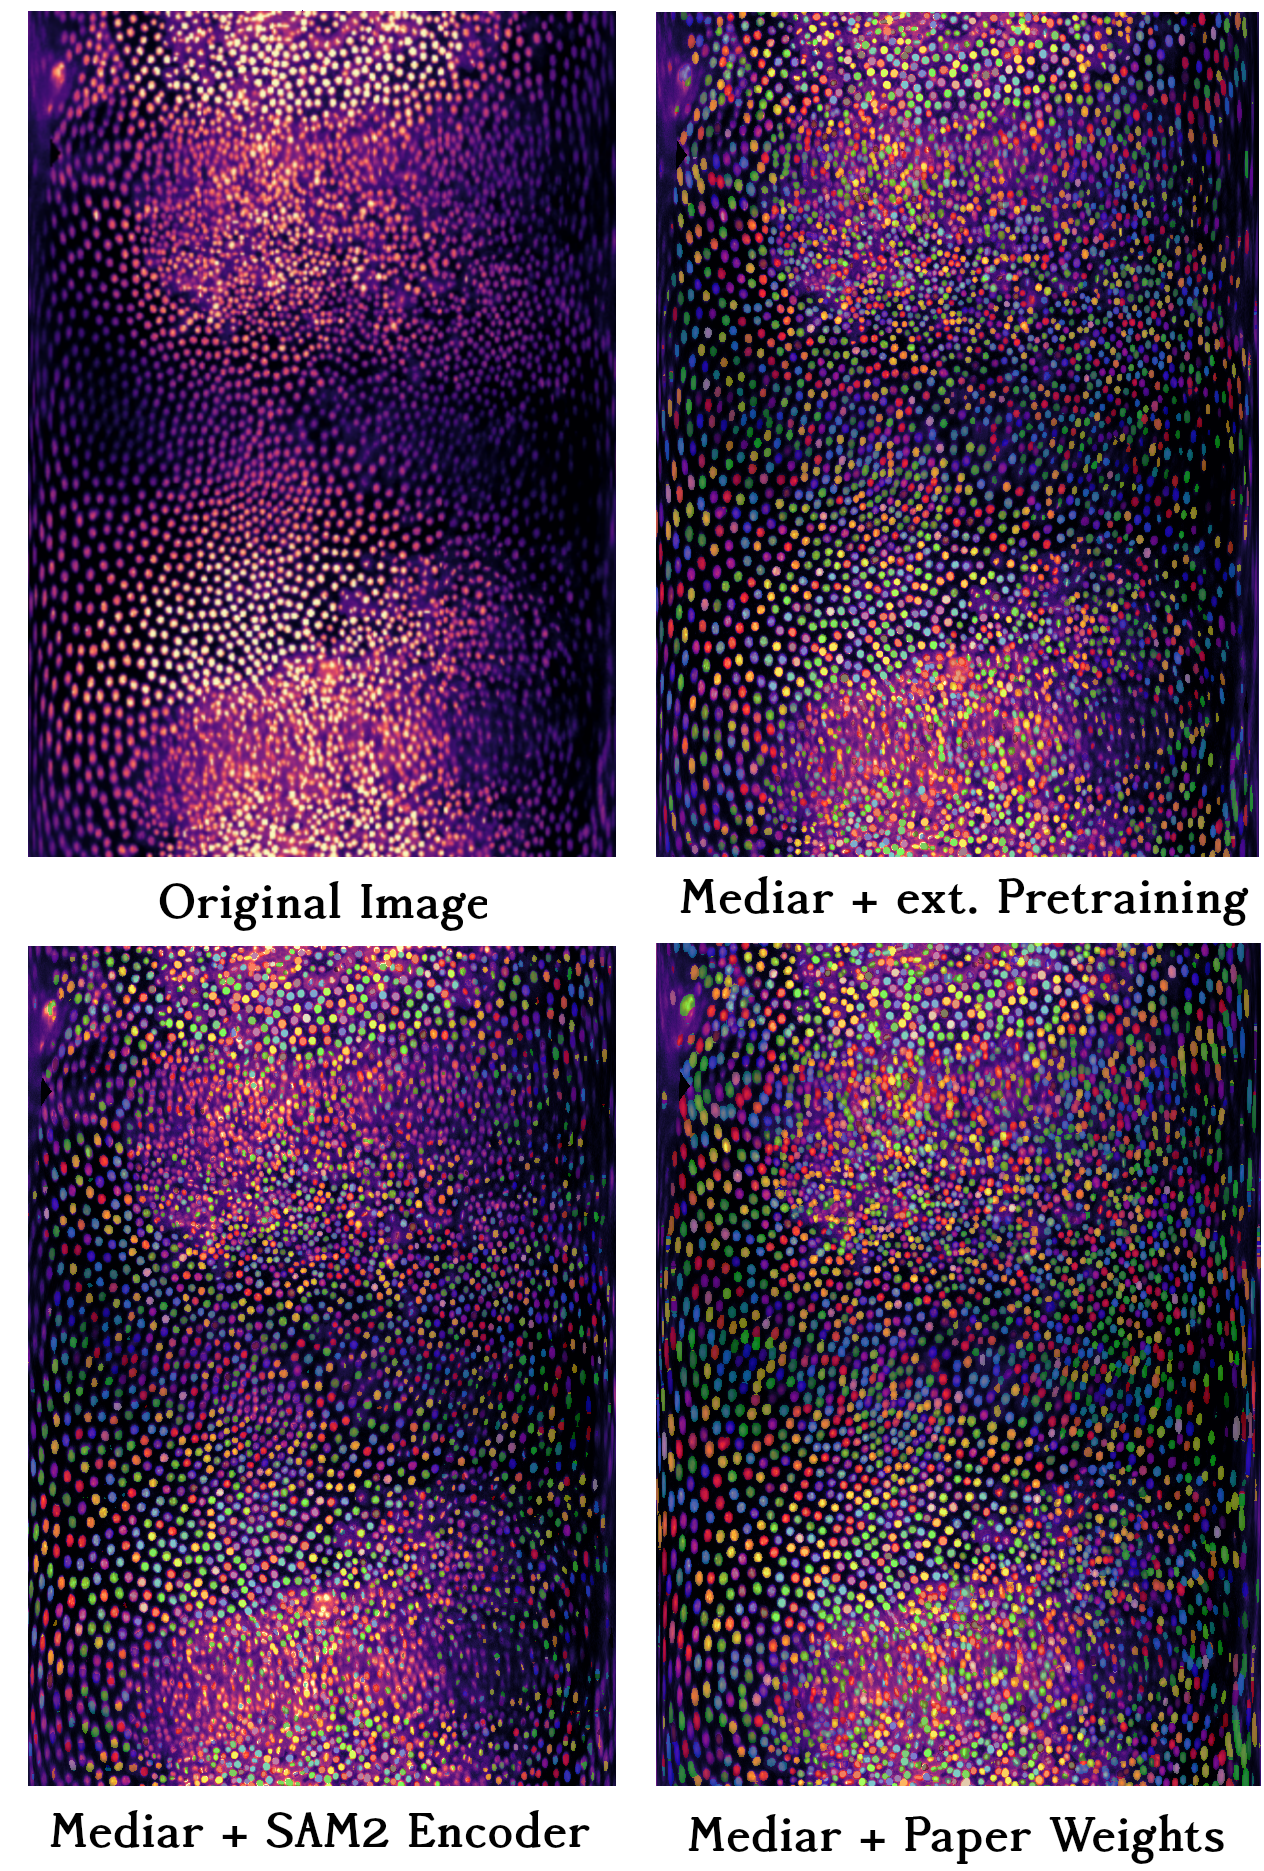
\includegraphics[width=0.95\textwidth]{Images/Appendix/TRIC_2D_slices.png}%
    }
    \caption{Prediction overlay on z-slice 12 of TRIC 02 sequence, timestamp 001. Mediar3D + ext. pretraining: 0.81 SEG @10 ROIs finetuning, Mediar3D + SAM2 Encoder: 0.65 SEG @10,000 ROIs finetuning, Mediar3D + paper weights: 0.81 SEG @10,000 ROIs finetuning}
    \label{fig:TRIC_2D_slices}
\end{figure}

\begin{figure}[!ht]
    \centering
    \makebox[\textwidth]{%
    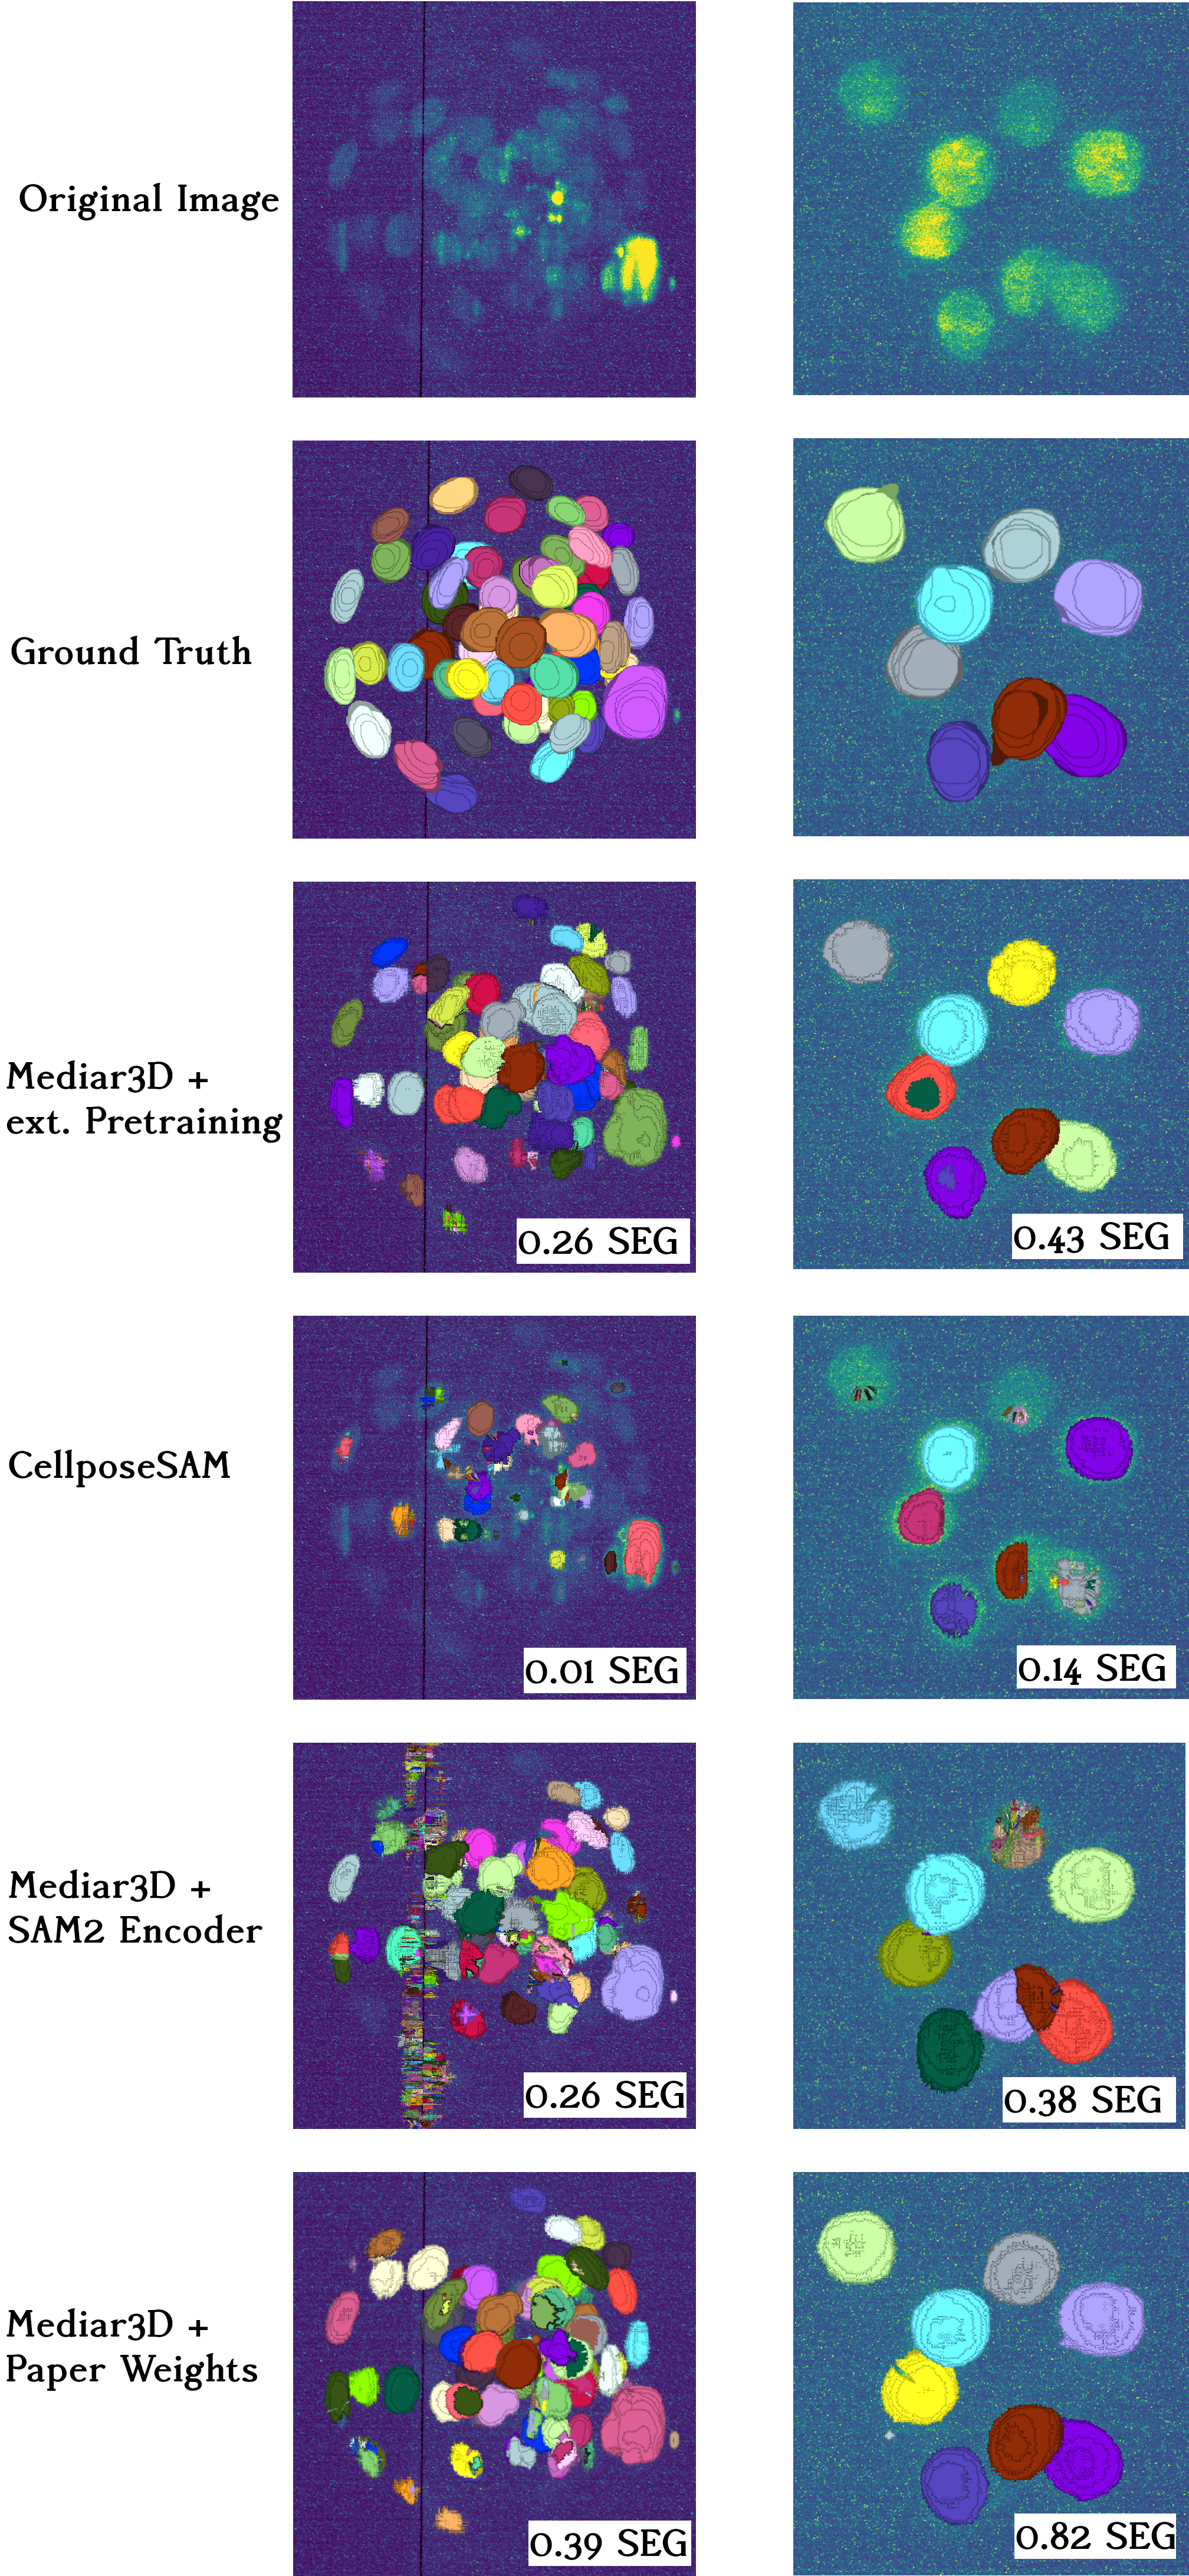
\includegraphics[width=0.64\textwidth]{Images/Appendix/Blasto_Result.png}%
    }
    \caption{BlastoSPIM result images, 3D rendered predictions overlaid with original image. Left column: 'Blast\_F2\_008', Right column: 'Blast\_H1\_009'. Model finetuning ROI stages and thresholds were manually selected for best case per model.}
    \label{fig:BlastoResults}
\end{figure}

\begin{figure}[!ht]
    \centering
    \makebox[\textwidth]{%
    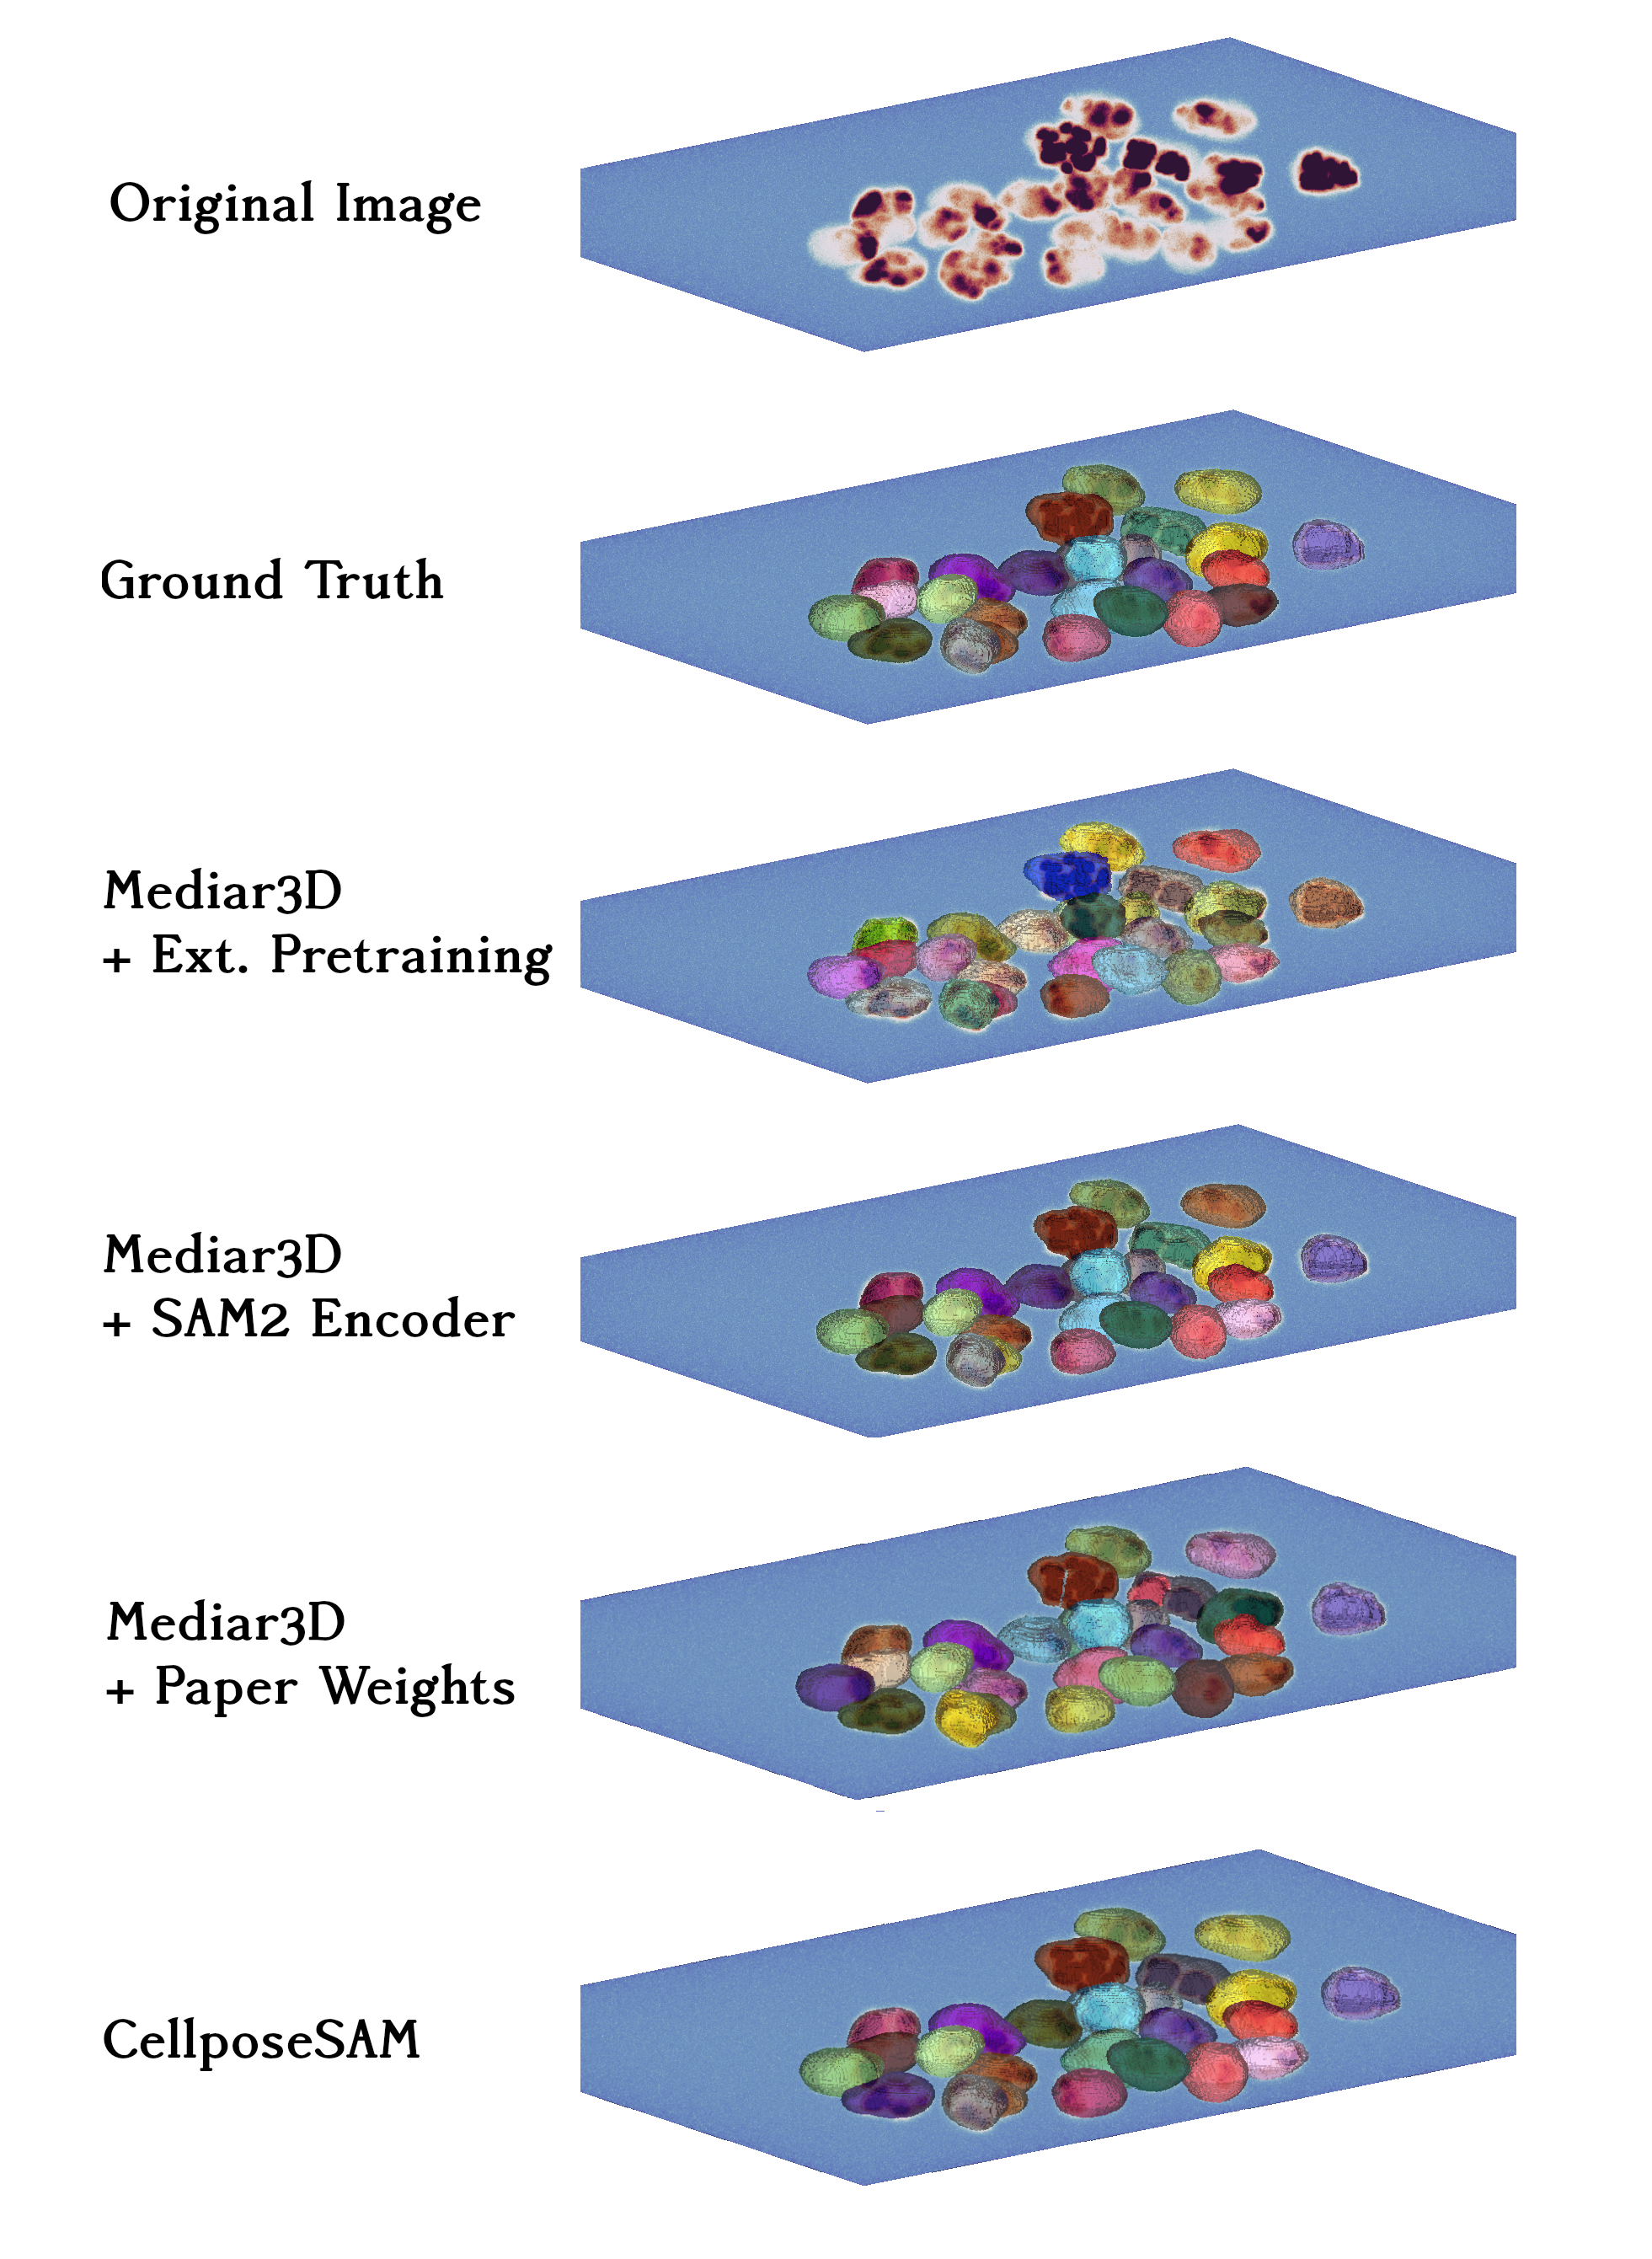
\includegraphics[width=0.98\textwidth]{Images/Appendix/SIM_results.png}%
    }
    \caption{Synthetic CTC result images, 3D rendered predictions overlaid with original image. All models were trained on 100000 ROIs and were evaluated on a cellprobability threshold of 0.5. As statistics of the 01 and 02 sequences correlate a lot, all models achieved SEG scores around 0.85-0.90. }
    \label{fig:SimResults}
\end{figure}







